% !TEX TS-program = pdflatex
% !TEX root = ../ArsClassica.tex

%************************************************
\chapter{La Composizione}
\label{chp:La Composizione}
%************************************************

Durante questi anni di accademia ho trasformato il mio rapporto con la composizione e il metodo di approccio agli strumenti e alle forme musicali. Dapprima ero in balia di un lungo
Il mio approccio alla composizione 
Come ogni mio attuale approccio a livello compositivo, ho cercato di creare una cellula di suoni disposti orizzontalmente, per poi lavorare sulla parte contrappuntistica. Dato che il nuovo strumento non ha pitch definiti � stato complicato lavorare su una cellula che al finire del suo svolgersi si potesse definire conclusa. Difatti ho cercato degli stratagemmi musicali, come gli accenti o la ricerca di determinati effetti timbrici (ad esempio attivazione di armoniche sugli estremi delle molle) che potessero diventare dei gesti musicali, sia a livello grafico che a livello d'ascolto. L'insieme di accento o di un numero determinato di gesti, vanno a formare le mie cellule ritmico-melodiche che interagiscono con la materia di cui � composta Sp.I.R.E. e quindi sempre in un rapporto 1:1 tra il ferro armonico delle placche e il metallo armoniche delle molle. Ogni cellula si sovrappone poi ad altre cellule simile in piccoli inserti contrappuntistici fatti di dilatazioni o restrizioni temporali del materiale sonoro. \\ 
Le cellule ritmiche sono formate da 7, 6, 5 e 11 eventi. La numerologia � legata al numero delle lettere che compongono nome e cognome dell'autore della poesia (7 = A-n-t-o-n-i-n, 6 = A-r-t-a-u-d), al numero delle sillabe del suddetto nome+cognome (5) e dal numero dei versi della poesia (11) sopra citata. \\
A livello compositivo compaiono delle cellule ritmiche che vanno a confluire in grossi nubi sonore. L'attinenza tra la scrittura e il gesto a volte � slegata, ma le piccole note e la tendenza ad una continuit� ?notazionale? porta l?esecutore-performer a capire in quali punti vanno gestiti dei continuum. \\
Su ogni continuum vanno a frammentarsi altre cellule ritmiche. Ogni cellula si ripete, ma con piccole variazioni temporali, ogni gesto � riconosciuto sia nella semiografia che dal timbro percepito.
Sar� poi l?elettronica a legarsi agli accenti e agli incontri verticali delle varie cellule ritmico-melodiche. Si noter� poi, durante la performance, che alcune scelte gestuali presenti in partitura, sono connesse ad un movimento esclusivamente performativo: quasi teatrale.\\
Entrando nel merito della stesura compositiva, vado a sottolineare alcune peculiarit� del movimento orizzontale e verticale delle voci. \\
Le varie parti di modulazione di frequenza e le interazioni ritmiche si incastrano seguendo un movimento verso le frequenze pi� alte. Se dall'inizio notiamo un'eccitazione delle sub-armoniche, qualit� tipica della natura delle molle, in seguito si � spinti verso frequenze sempre pi� alte, cercando di andare di pari passo con una lettura temporale della poesia di Artaud: dalla vista dal basso verso l'alto degli astri (\textit{verres o� cuisent les cerveaux / le ciel fourmillant d'impudeurs}) la notazione si erige, come grande rosone, verso armoniche generate sia dal materiale metallico composto dalle molle, sia da quello delle piastre. Si va ad indagare, quindi, \textit{nello} strumento (tramite una scrittura prettamente legata all'universo delle percussioni) sia textit{sullo} strumento (tramite l'utilizzo dell'elettronica). Tengo a sottolineare che l'amplificazione � colonna portante di tutto il brano, dato che tutte le elaborazioni e i contributi dell'elettronica sono diffusi esclusivamente tramite gli attuatori. L'amplificazione e qualunque elettronica a supporto della performance sono amplificate dai piezoelettrici e dai microfoni omnidirezionali. \\
Ogni contributo � un valore aggiunto a Sp.I.R.E. che si lascia 
\\
\\
La partitura ha come oggetto principale di scrittura, il processo con il quale sono stati ricercati i suoni: ogni gesto descritto graficamente, rappresenta il processo del timbro e della forma con la quale si vuole arrivare verso determinati frasi musicali, sia di natura percussiva che di natura timbrica.

\section{Materiali sonori}
\addcontentsline{toc}{section}{Materiali sonori}
Vitres de son � stata composta quindi su un sistema che si pu� definire sia \textbf{Acustico} che \textbf{elettronico}. \footnote{Acustica musicale e architettonica a cura di Sergio Cingolani, Renato Spagnolo UTET, 2004 Torino p. 3}

Tra i primi appunti ci furono molte stesure di una partitura che potesse legarsi: 
\begin{itemize}
\item{teatrale}
\item{tmondo sonoro}
\item{interazione}
\end{itemize}

Suoni di sfondo si adagiano su una superficie. Da l� diventano protagonisti, dal paesaggio sonoro, da un soundscape, fatto di piccoli grattati in \textbf{\textit{ppp}}, emergono forme che si incastrano con le figure ritmiche, ovvero le sillabe dei versi della poesia. Come se prendessero la forma di piccoli respiri, dati dalla lettura delle parole del poeta. Appare un \textit{dramma}, un enorme piaga che sottolinea Artaud in tutta la sua poetica giovanile e nei suoi lavori teatrali: non c'� pi� linguaggio parlato, divincolato dalla struttura principale di diffusione orale, ma solo suono. La musica, come la poesia, da suono di parole recitate, diventa figure ritimiche. \\
Nello stesso modo con il quale si applicano modifiche a livello di velocit� di emissione delle sillabe durante una recitazione, cos� ho cercato di dar vita a delle variazioni nelle strutture ritmiche che si fondo con l'universo sonoro sottostante e vengono inghiottite dal soundscape. Ci� � reso possibile dalla natura del materiale: ogni passaggio delle dita o unghie sulle spire delle molle crea dei micro-glissati che formano maglie di suono che si fondono con le elaborazioni del live electronics. Ad un tratto appare, su frequenze gravi, una modulazione di frequenza. Questa FM, al suo interno ha dei piccoli movimenti spettrali, legati ad altrettanto piccole variazioni di parametri interni. Come affermava Xenakis:
\begin{quotation}
Una moltitudine di brevi \textit{glissandi} pu� dare l'impressione del continuo, come anche una moltitudine di \textit{pizzicati}\footnote{Iannis Xenakis, \textit{Universi del suono, Scritti e interventi 1955-1994} (a cura di Agostino Di Scipio), Ricordi S.r.l. e LIM Editrice S.r.l., 2003 \\}.
\end{quotation}




\section{Idea ritmico-melodica}
\addcontentsline{toc}{section}{Idea ritmico-melodica}

Affezionato alla poetica di Cage 
Le figure ritmiche servono a dare alla composizione un andamento strutturale. Ovvero, anche se molte figure non sono legate ad un preciso \textit{ictus}, servono comunque a creare degli incontri, ad esempio tra elettronica e parte strumentale o il movimento verticale di pi� voci. in \textit{Vitres de Son} in queste figure ritmiche sono nascoste le sillabazioni dei versi della poesia di Artaud, cercando di far intuire un andamento "vocale" delle parti. \\
Ho considerato utili tecniche di scrittura contemporanea legate al mondo degli idiofoni e all'universo dei cordofoni. \\
Per quanto riguarda la notazione, ho trovato, nel libro sulla semiografia contemporanea di Luigi Donora\footnote{Luigi Donora, \textit{Semiografia della nuova musica}, }, molte delucidazioni sulla creazione di figure ritmiche e simboli che potessero al meglio rappresentare il mio fine compositivo. Per fine compositivo intendo la possibilit� di creare determinati timbri, riportando notazioni non canoniche ma che facessero capire la tipologia di gesto da utilizzare in un determinato frammento. Durante la stesura della partitura ha cambiato forma diverse volte. La prima partitura, infatti, era stata creata direttamente su una serie di pentagrammi, dove il si sopra al do centrale stava a simboleggiare il centro della molla e il movimento verso l'alto e verso il basso delle note rappresentava rispettivamente un movimento verso destra e verso sinistra (fig. ?)
\begin{floatingfigure}{10cm}
\mbox{\epsfig{file=fig_ritmica.jpg,width=9cm}}
\small{\caption{\textit{particolare}}}
\end{floatingfigure}

Le figure ritimiche servono a dare alla composizione un andamento strutturale. Ovvero, anche se molte figure non sono legate dad un ictus preciso, servono comunque a creare degli incontri, tra elettronica e parte strumentale o in alcuni punti nell?incontro verticale dipi� voci. All?interno di queste figure ritmiche sono nascoste le sillabazioni dei versi della poesia di Artau che prende
il nome del pezzo e rendono possibile una?vocalit�? della composizione.

Ho considerato utili tecniche di scrittura contemporanea legate al mondo degli idiofoni e all'universo dei cordofoni. Per quanto riguarda il pentagramma, nella prima stesura era stato utilizzato per il movimento sulle corde, come in figura, si identifica il movimento da sinistra verso destra, con il movimento dal basso verso l'alto. In seguito, ogni movimento sul pentagramma, ogni forma che produceva un suono differente, si � trasformata in simbolo: ogni simbolo rappresenta quindi un gesto che si sviluppa in un determinato suono con un suo timbro specifico.
Saranno considerate utili tecniche di scrittura contemporanea, legata al mondo delle percussioni per lo strumento di nuova creazione. Il pentagramma diventa la base di un movimento sull'asse orizzontale dello strumento. Il pentagramma con centro sul Si sopra al Do centrale, nella prima stesura, ed un uno rigo unico con centro nel rigo stesso nella seconda, rappresentano graficamente una determinata molla che sar� nominata in legenda con la lettera M. Per rendere pi� semplice ogni movimento e ogni incastro ritmico, ho redatto degli esempi che vengono esplicati in legenda tramite una didascalia, cos� da migliorare l'approccio con la partitura e di conseguenza con l'iper-strumento.

\section{Gestualit�}
\addcontentsline{toc}{section}{Gestualit�}

Sar� quindi il gesto ad essere la base della prosodia interna, ogni legame con il gesto successivo sar� studiato per dare un movimento sia alle voci, che possono essere fino a 3 simultanee, come si nota nell'ultima pagina della partitura, dove la punta dell'arco si muove su una placca (P2), il centro dell'arco si muove su M5 e la base dell'archetto percuote M4 chiudendo in un crescendo dinamico.
L'utilizzo di simboli vicini al mondo della musica classica mi ha aiutato ad adeguare uno strumento del quale non abbiamo letteratura, verso una nuova scrittura, tutto ci� � la base poi della musica contemporanea, ovvero, ogni nuovo gesto � l'evoluzione di un gesto appartenente a musica pi� antica. Alcuni movimento dell'archetto infatti stanno a simboleggiare i gesti della mano o dell'archetto, come avveniva in passato per la musica gregoriana, con i melisimi legati al movimento delle mani dei direttori di coro della tradizione.

\section{Macro-forma}
\addcontentsline{toc}{section}{Macro-forma}

Il lavoro � svolto sulla poesia di Artaud. Come se ogni gesto si collegasse ad una parafrasi immaginifica e musicale della poesia del drammaturgo francese. \\

\begin{quotation}
\textit{Vitres de son o� virent les astres \\
verres o� cuisent les cerveaux \\
le ciel fourmillant d'impudeurs \\
d�vore la nudit� des astres. \\ \\ \\}
\end{quotation}





\section{La legenda}
\addcontentsline{toc}{section}{La legenda}
La partitura si apre con il progetto di Sp.I.R.E., per poterlo riprodurre ed utilizzare materiali affini.\\
Per facilitare la lettura della partitura elettroacustica, ho preferito dividere la legenda in quattro blocchi fondamentali:
\begin{itemize}
\item{Il primo blocco comprende la tipologia di battenti, utilizzati anche nella musica classica, ma \textit{numerati}, per facilitare i cambi in partitura, dato che per ogni battente abbiamo un'eccitazione diversa delle molle e un timbro differente.}
\item{Il secondo blocco delinea la notazione e la simbologia presente in partitura}
\item{Il terzo blocco ha al suo interno degli esempi che facilitano lo studio degli incastri ritmici}
\item{L'ultimo blocco comprende tutti i simboli e i gesti legati all'elettronica (pedali, variazioni di parametri, elaborazioni)}
\end{itemize}


\begin{center}
\begin{minipage}[c]{1.\textwidth}
\includegraphics[width=0.4\textwidth]{legenda1.jpg}
\end{minipage}
\end{center}


\begin{center}
\begin{minipage}[c]{1.\textwidth}
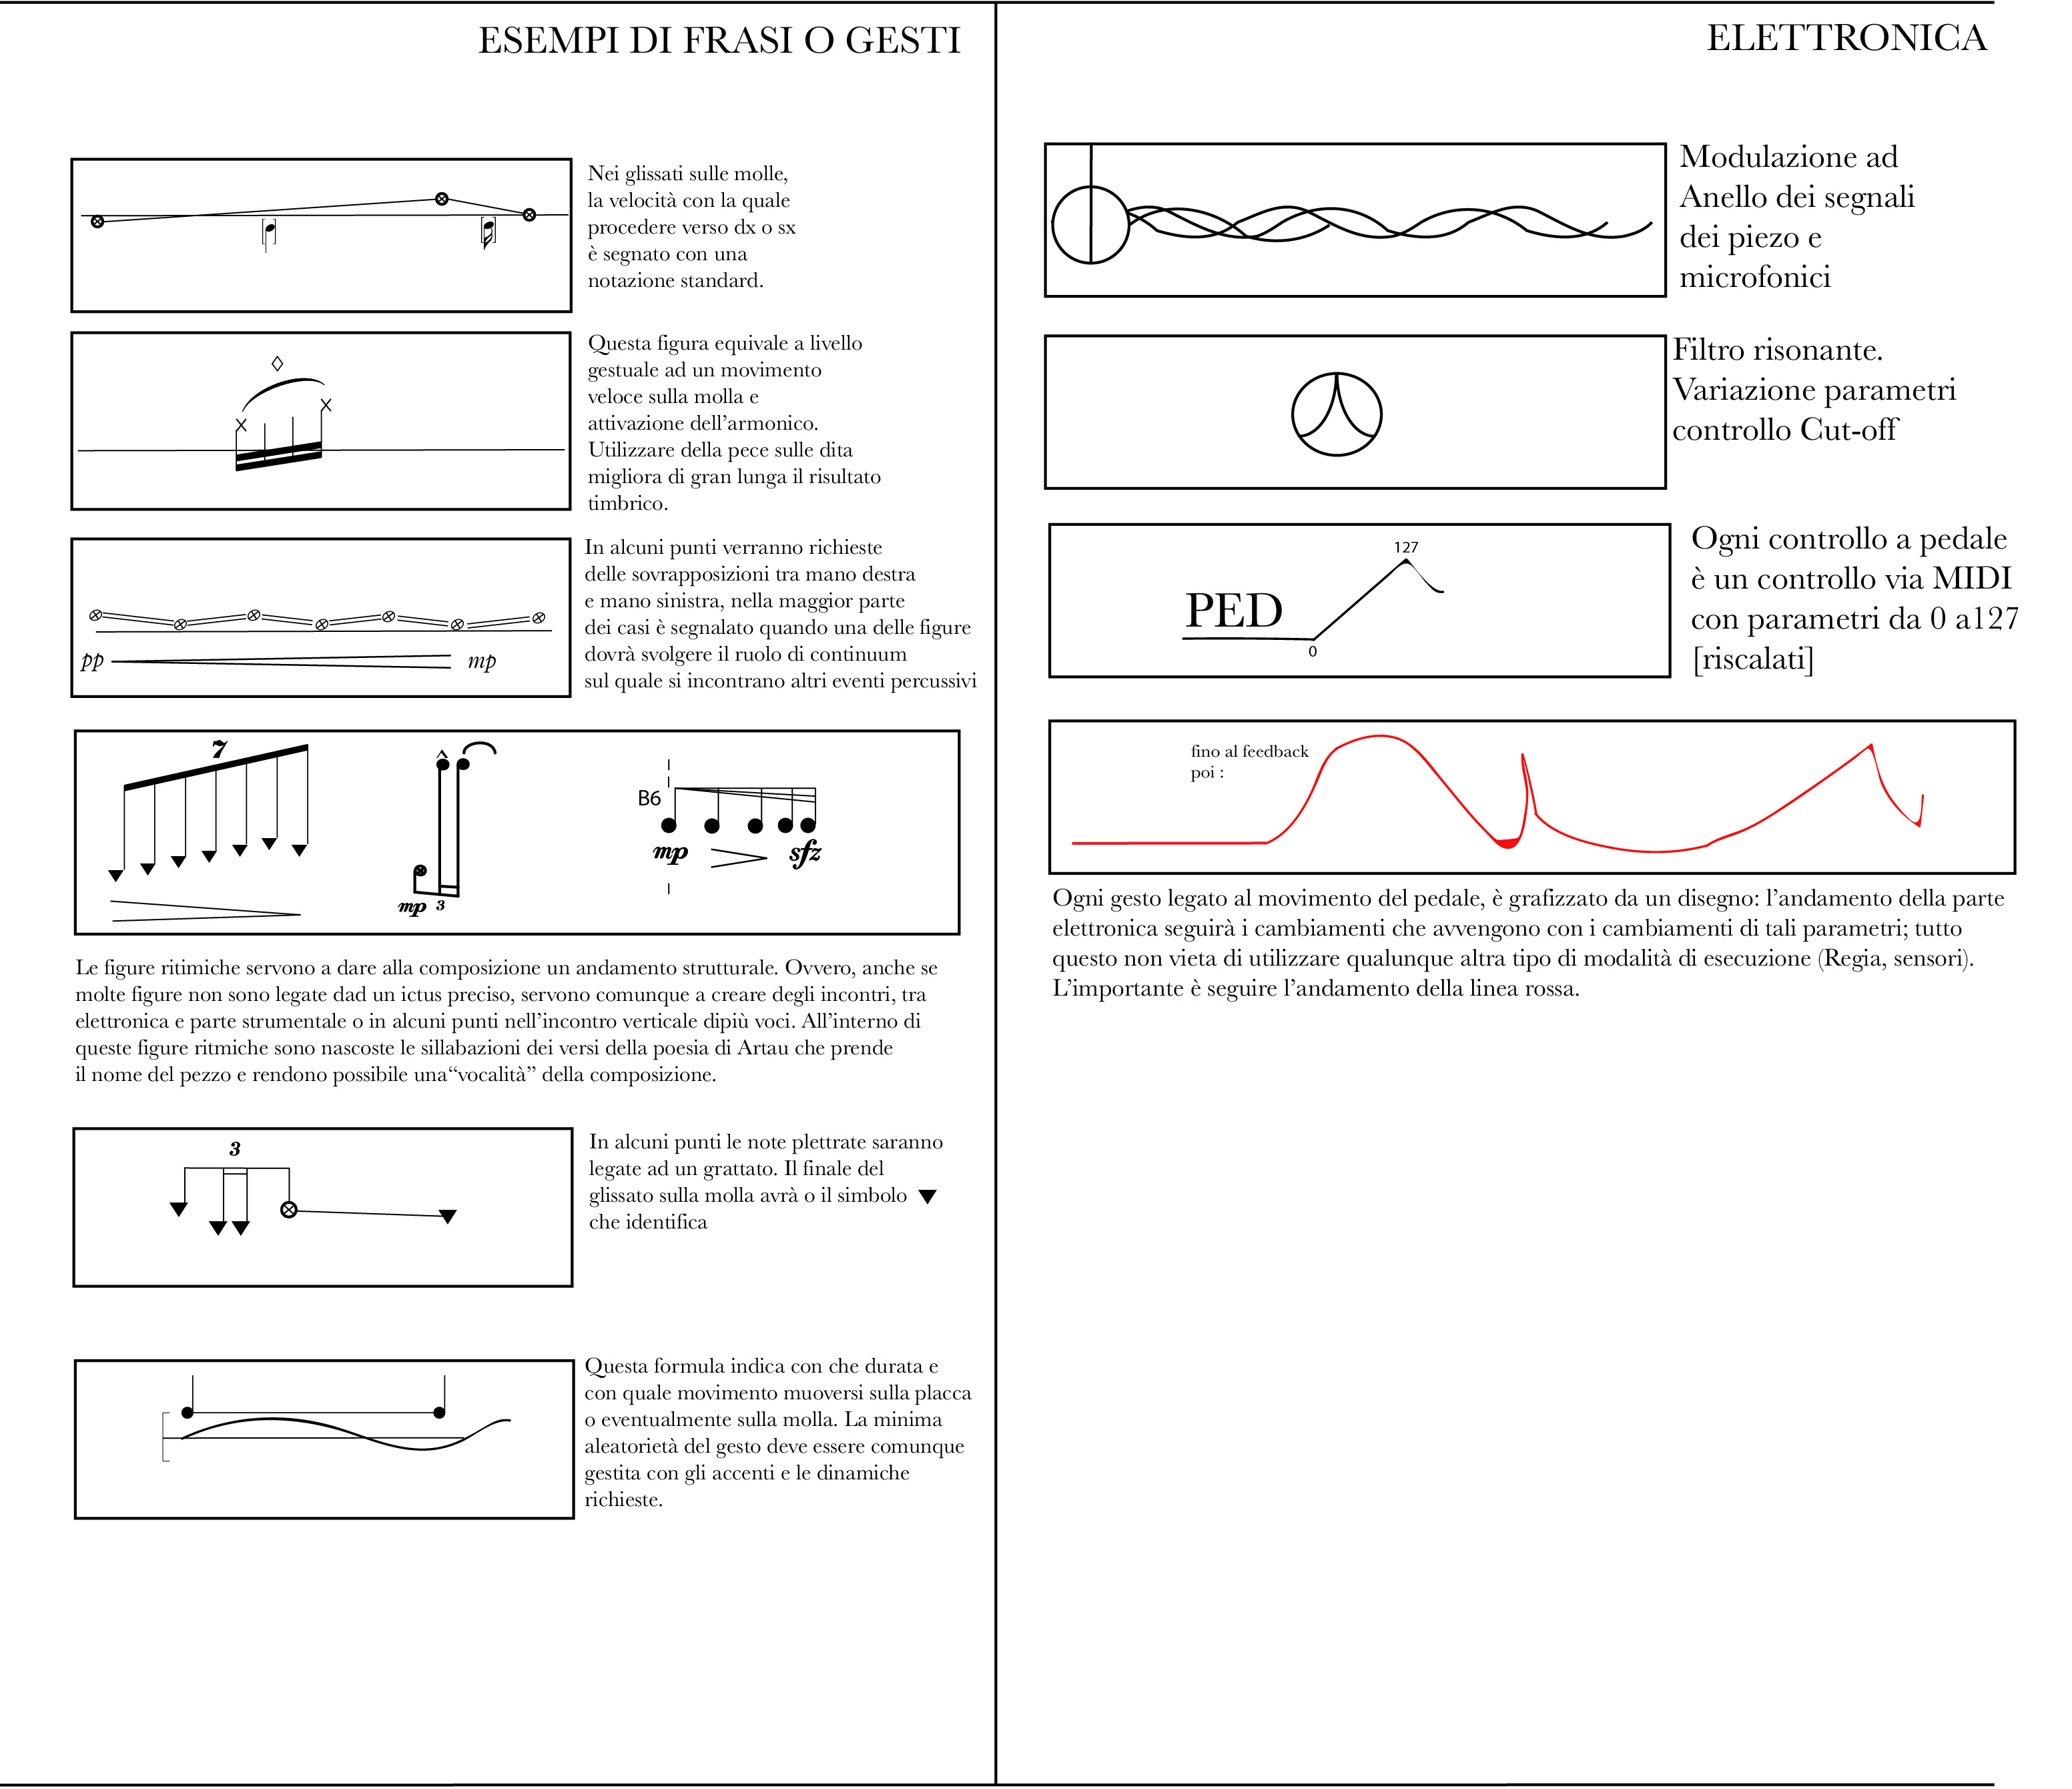
\includegraphics[width=0.6\textwidth]{legenda2.jpg}
\end{minipage}
\end{center}


\section{Algoritmi}
\addcontentsline{toc}{section}{Algoritmi}
\begin{center}
\begin{minipage}[c]{1.\textwidth}
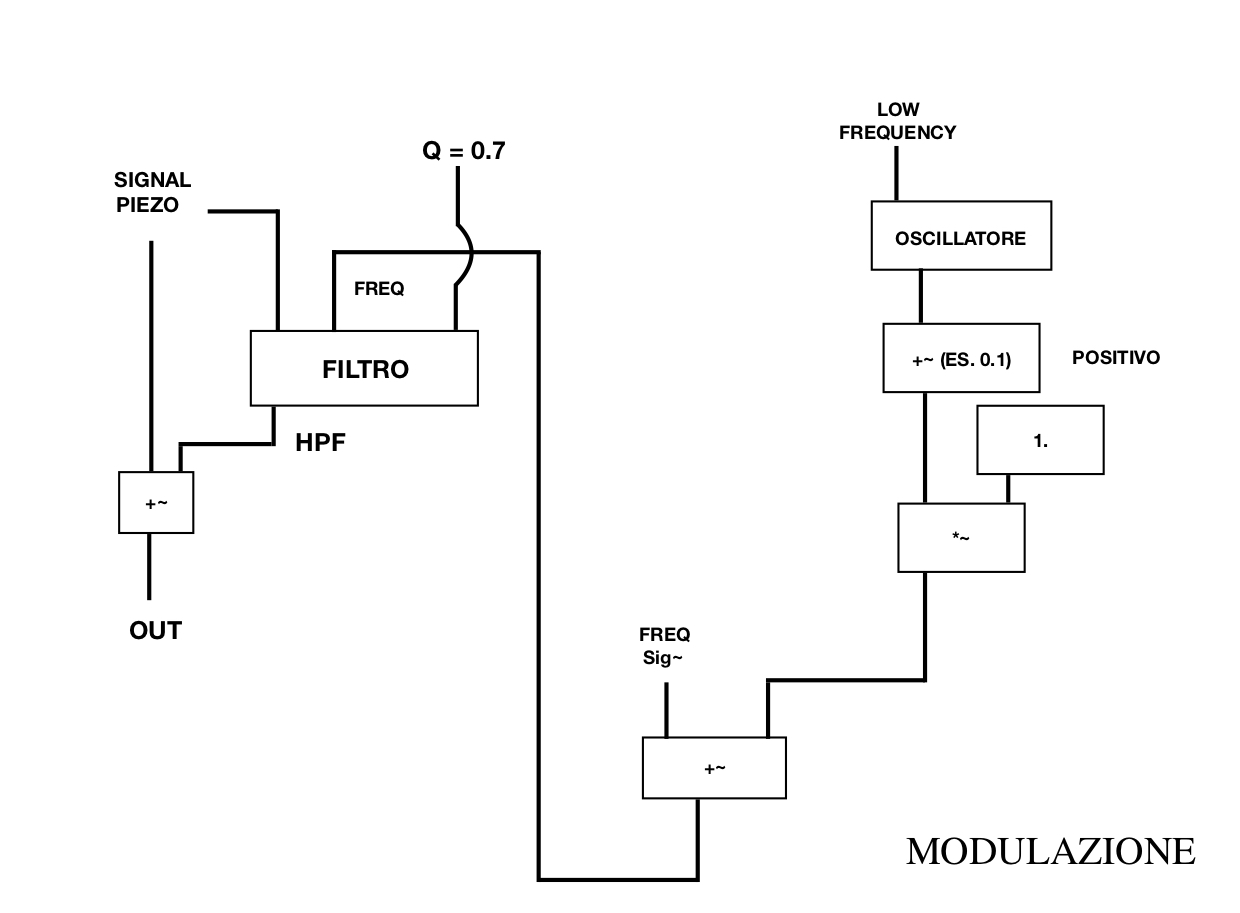
\includegraphics[width=1.\textwidth]{algo_1.jpg}
\end{minipage}
\end{center}
\begin{center}
\begin{minipage}[c]{1.\textwidth}
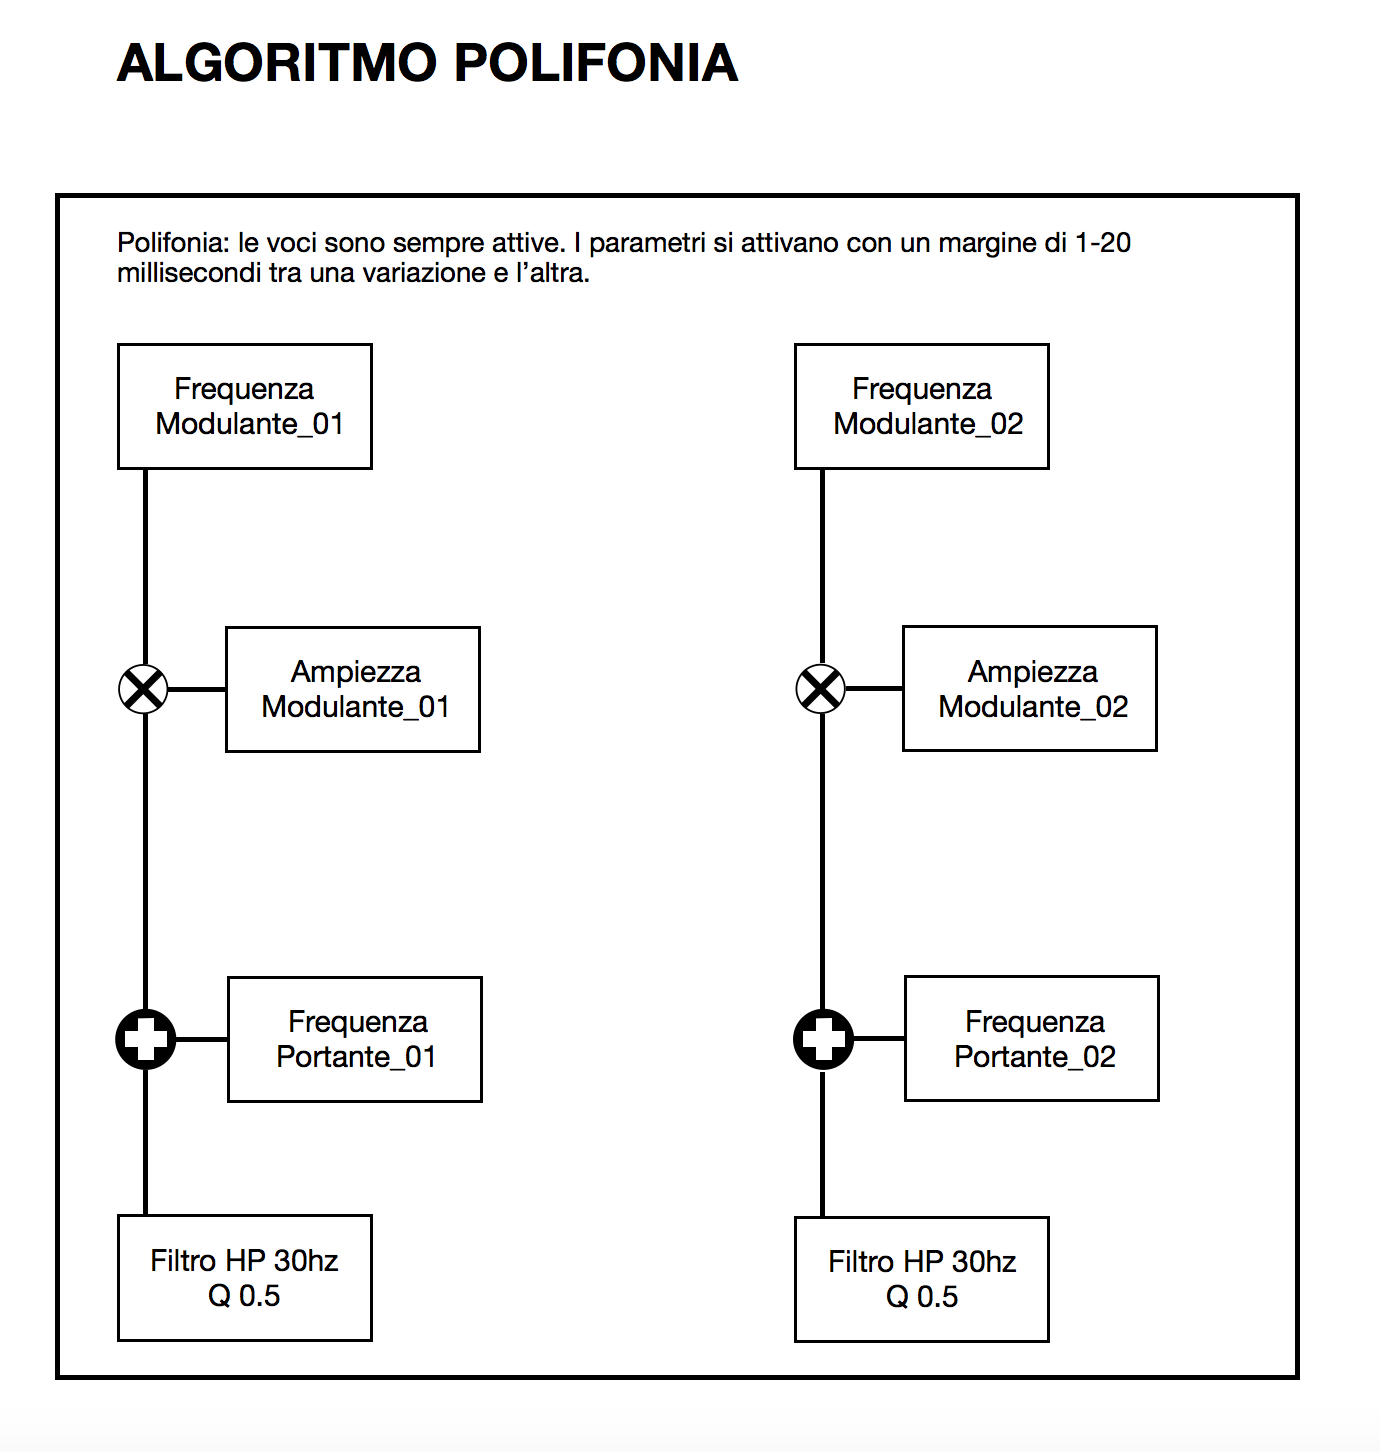
\includegraphics[width=1.\textwidth]{algo_2.jpg}
\end{minipage}
\end{center}


\section{Pedaliera}
\addcontentsline{toc}{section}{Pedaliera}

Pedaliera. Dopo aver studiato il funzionamento ho notato che ogni pulsante numerato era assegnato ad un NOTE on, come una normalissima pedaliera midi per organo. La fortuna � che ogni pulsante equivale a note inerenti al numero presente sulla pedaliera (es. note-on 1 = tasto 1 pedaliera). Quindi essendo identiche, ho solo dovuto trasformare ogni note-on in un ?lancio-scena? sul mio software di utilizzo (max-msp). Questo mi ha facilitato lo studio con il performer che pu� riprovare ogni scena senza dover ripetere temporalmente la sequenza in partitura, ovvero pu� passare ad esempio dalla scena 1 alla scena 6 senza dover ripercorrere tutte le scene presenti tra quelle menzionate. Questo facilita la prova per ogni singolo rigo.
